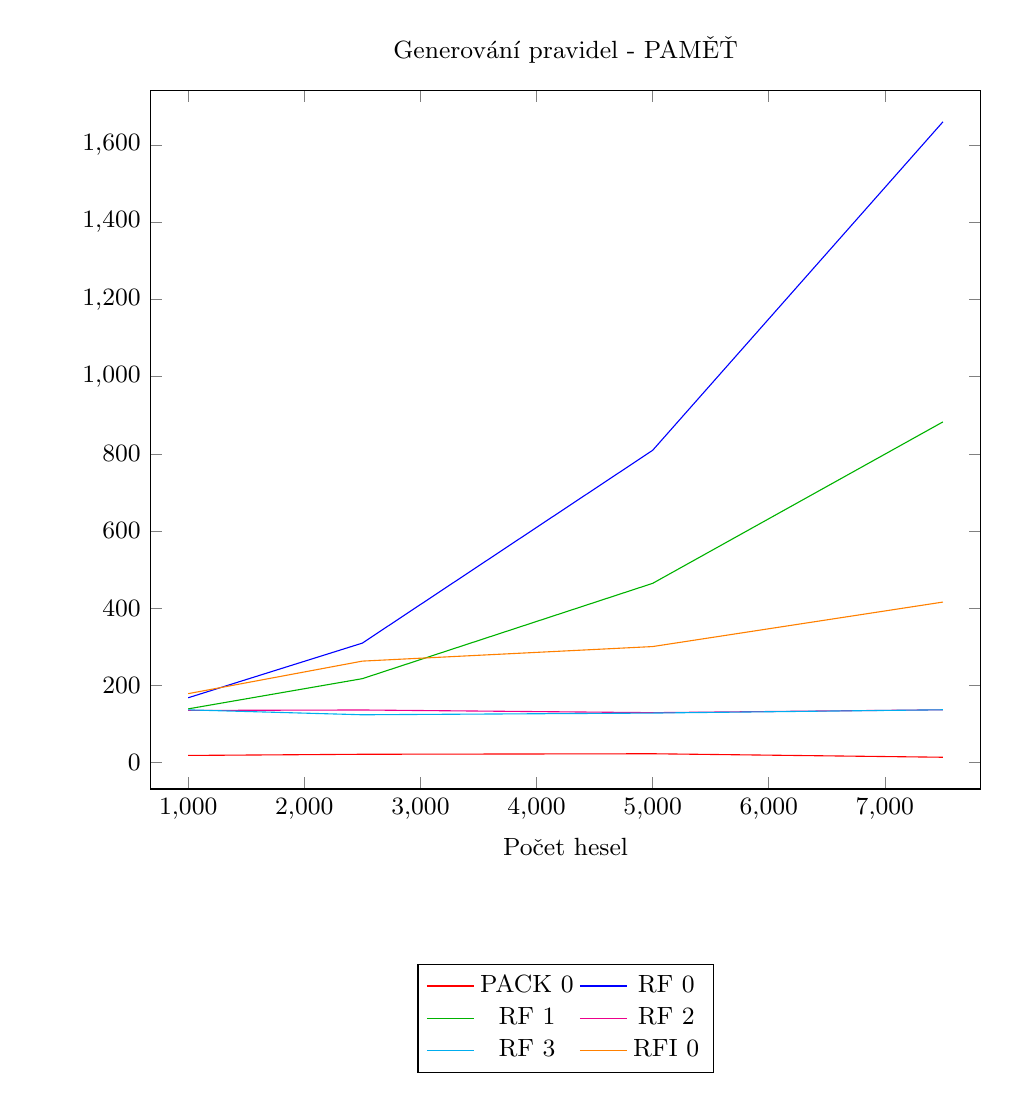
\begin{tikzpicture}
  \begin{axis}[
    width=\linewidth, 
    every axis/.append style={font=\small},
    title={Generování pravidel - PAMĚŤ},
    xlabel={Počet hesel},
    ylabel={\phantom{Paměť [MB]}},
    legend style={
      at={(0.5,-0.25)},
      anchor=north,
      legend columns=2,
    },
    enlargelimits=0.05,
    scaled y ticks = false,
    scaled x ticks = false,
    cycle list={
     {red},
     {blue},
     {green!70!black},
     {magenta},
     {cyan},
     {orange},
     {violet},
     {purple},
     {gray},
     {darkgray}%
    }
    ]
    
    \addplot coordinates {
      (1000, 18.12) 
      (2500, 21.17) 
      (5000, 22.49) 
      (7500, 13.45) 
      }; % PACK 0
    
    \addplot coordinates {
      (1000, 167.61) 
      (2500, 309.29) 
      (5000, 808.98) 
      (7500, 1660.39) 
      }; % RF 0
    
    \addplot coordinates {
      (1000, 138.82) 
      (2500, 217.15) 
      (5000, 464.19) 
      (7500, 882.64) 
      }; % RF 1
    
    \addplot coordinates {
      (1000, 134.79) 
      (2500, 135.93) 
      (5000, 129.0) 
      (7500, 136.43) 
      }; % RF 2
    
    \addplot coordinates {
      (1000, 136.26) 
      (2500, 123.54) 
      (5000, 127.96) 
      (7500, 136.48) 
      }; % RF 3
    
    \addplot coordinates {
      (1000, 178.27) 
      (2500, 262.61) 
      (5000, 300.34) 
      (7500, 415.66) 
      }; % RFI 0
    
    \legend{PACK 0, RF 0, RF 1, RF 2, RF 3, RFI 0}
  \end{axis}
\end{tikzpicture}